% !TEX root = main.tex

\section{シーケンス制御の基礎実習}

\subsection{実験目的}
シーケンス制御とは,あらかじめ決められた順序または手続きに沿って制御の各段階を逐次進めていく
制御方法のことで,例えば炊飯器の制御が該当する.炊飯器の場合は,
予約設定から炊き上がりおよび時間を予約設定を行うまでの流れがあらかじめ決められており,
一方向にしか制御は進まない.

ひとつの作業を終了することで,次の作業に移ることから,
そのような制御方法を順序制御と呼ぶ.他に,時間によって作業を切り替える時間制御,
あらかじめ決められた作業の中から現在の条件に見合う作業を選択する条件制御など,
シーケンス制御の内部にして様々な制御方法が存在する.

\begin{itemize}
  \item 順序制御の例:自動販売機
  \item 時間制御の例:信号機
  \item 条件制御の例:洗濯機
\end{itemize}

本実験では,FAシステムを構築する前の準備訓練として,
オムロン株式会社寄贈のベーシックFAキットを用いて
シーケンス制御の基礎を学習することを目的とする.

\subsection{実験装置の概要}

本実験では,ベーシックFAキットを使用する.
また,このベーシックFAキットには拡張パーツボックスが付いている.
これらのパーツ(センサーやタイマー等)についての詳細は次章で述べる.

図1.4にベーシックFAキットの内部配線図を示す.
FAキットの入力はAC 100 [V]とし,内部のパワーサプライによってDC 24 [V]に変換されている.
よって,以降で使用するパーツ(センサーやタイマー等)はDC 24 [V]駆動の製品である.

キット本体は主に,タイマの調整スイッチ,SW1〜SW4までの4つの押しボタンスイッチ,
コンベア制御用の切り替えスイッチ,L1〜L3までの表示灯,およびコンベアで構成されている.
ただし,SW4だけスイッチの種類が違うことに注意すること.

次に,このベーシックFAキットの基本的な使用方法について,最も単純な使用例を挙げて説明する.
例えば以下の手順に従い,SW1を押せばL1が点灯する機能を作ることにする.
\begin{enumerate}
  \item まず,背面に入っているコネクトを接続し,クレーターを上げる.
  \item 次に「+24V端子とスイッチ1」,「スイッチ1と表示灯1」そして「表示灯1と-V」を各ケーブルで接続する.
  \item 最後に電源を入れスイッチ1を押せば表示灯1が点灯する.
\end{enumerate}

なお,赤いリード線が+24Vに対応することを推奨するが,配線の見直し時に便利なため,
-Vには青,それ以外は黄を使うことを推奨する.

\subsection{シーケンス制御に必要な電子機器}

本章では,シーケンス制御に必要な電子機器について述べる.ただし,これらの知識があるならば,本章を読み飛ばして次章に移っても差し支えない.

\subsubsection{スイッチとリレー}
本実験の基礎となるのはリレーシーケンス制御である.
リレーを用いたシーケンス制御のことをリレーシーケンス制御と呼び,
通常シーケンス制御といえばこれを意味する.
リレーとは「電流によって制御可能なスイッチ」のことで,
これを用いることで回路内の電流の進行方向を制御し,出力先を任意に設定することが可能である.

リレーの種類としては,有接点リレーと無接点リレーが挙げられる.
有接点リレーは,主に電磁リレーのことを指し,電流によって磁力を生じさせてスイッチをON/OFFさせる.
一方,無接点リレーは,ダイオード,トランジスタなどの半導体を用いてON/OFFを行うものである.
また,無接点リレーを用いた制御では論理演算を行うために論理シーケンス制御と呼ばれる.
しかし,扱える電流・電圧の範囲が狭く,直接接続制御には不向きである.
また,PLCが主流である現在では,回路の変更が容易でない,などの理由から利用される機会は少なくなっている.
本実験でもリレーは基本的な有接点リレーを用いることにする.

\paragraph{a 接点スイッチ}
a接点スイッチとはボタンを押しこむことで端子間が導通するスイッチのことであり,
通常時は接続(開放)されているNO (Normally Open) 接点ともいわれる.
ボタンを押している時だけ導通し,離せば接続されることに注意すること.

\paragraph{b 接点スイッチ}
b接点スイッチとはボタンを押しこむことで端子間が絶縁するスイッチのことであり,
通常時は導通しているNC (Normally Close) 接点ともいわれる.ボタンを押している時だけ端子間は開放され,
離せば導通することに注意すること.

\paragraph{c 接点スイッチ}
c接点とはa接点とb接点の両方の特性を併せ持つスイッチである.
通常はb接点とCOM (common),押しこむことでa接点とCOMが導通することになる.
リレーでは,このc接点の機能を備えているものが多く用いられている.
本実験で使用するリレーもc接点を持っている.また実験で使用するマイクロスイッチもc接点である.

\paragraph{リレー}
電磁コイルに電流を流すことで磁界が発生し,可動鉄片に磁力がかかる.
それによって,可動鉄片がb接点から離れ,a接点と切り替え接点(COM)が導通する.
また,電磁コイルに電流を流すことを止めると,伸ばされていたバネによる力でa接点から離れ,
元のb接点と再び導通する.このようにリレーは,電流を流すことでON/OFF(a接点とb接点の切り替え)
が可能なスイッチの機能を持つ素子である.

リレーの端子において端子9〜12がCOMとなっており,端子1〜4がNC,端子5〜8がNOの役割を持つ.
端子14に+24V,端子13に-Vを入力するとリレーがONとなり,COMとNO端子が導通する.
なお,リレーは接続端子が付いたソケットに挿入して用いることで配線が容易となる.

\subsubsection{タイマ}
タイマとは,設定した時間を作り,その設定時間後に内蔵スイッチ(リレー)を切り替える機器のことである.
端子の配線についてはリレーと同様である.

また,本実験で使用するタイマH3YNには側面に4つのディップスイッチが付いている.
上2つのディップスイッチでタイマ時間の単位(1s, 10s, 1min, 10min)を変更することができる.
また下2つのディップスイッチで4つの動作モードが設定可能である.

\subsubsection{カウンタ}
カウンタとは数を数える機能を持った機器のことであり,設定値に達することで出力する機能を併せ持つ.
各端子の役割が設定されており,6番と9番が導通するとカウントアップ,6番と7番が導通するとリセットとなる.
また,3番はCOMの役割を持ち,設定値にカウント数が達するとNOの4番と導通,NCの5番が絶縁する.
タイマ同様,側面のディップスイッチによって動作の設定が可能である.
ただし,本実験では特に設定変更は必要ない.

\subsection{近接センサ}
近接センサとは,磁界や電界を利用して近づく金属に反応するセンサのことである.
茶色のケーブルに24 V,青色に0 Vを接続して動作させる.検知信号は,黒ケーブルから取り出せるが,
負荷(例えば表示灯)の0 V側と接続して用いる.

\subsubsection{光電センサ}
光電センサとは,可視光線や赤外線などの光を利用するセンサであり,応答速度が速い,
検出距離が長いなどの特徴を持つ.本実験で用意している光電センサには透過形,
回帰反射形,拡散反射形の三種類がある.

\subsection{シーケンス制御の基礎理論・シーケンス回路図}

本節では,シーケンス制御の基礎理論となるシーケンス回路図について述べる.
ただし,シーケンス制御についての知識があるならば,次章の実験内容に移っても差し支えない.

シーケンス回路図は制御における論理回路を表すものであり,電気回路図とは異なっており
,シーケンス回路図(あるいはリレー回路図など)と呼ばれる図面に対応する.
シーケンス回路図の基本となるシンボルは,これに応じた装置の動作方法が存在することを留意すること.

ここで,コイルの記号について少し詳しく述べておく.リレーのコイルとは,リレーの動作電源となる端子13, 14番のことである

また,タイマの出力はリレーと同様に接点やコイルを持っている.

\subsubsection{例題によるシーケンス回路図解説}
指導書図1.22にシーケンス回路図の例を示す.
SWは押しボタンスイッチ,Rはリレー,OUTは出力(例えば表示灯)を意味する.

この回路の動作は,SWを押すことでリレーのコイル(電磁リレーの場合)に電流が流れ,
磁力に反応してa接点がONとなりOUTに出力される.通常,電流は流れ続けるが,
左側が開閉しない限りGNDと考えスムーズな動作を行う.なお,図中の記号において接点は上が下,
下が上と直線的に作動する.

\subsubsection{シーケンス回路図における注意点}
シーケンス回路図を作成する上で以下のことに注意が必要である.
\begin{itemize}
  \item 出力,コイルの後には何も設置しない
  \item 出力,コイルを直列に設置しない
  \item 接点なしで直接出力しない
  \item 短絡させない
\end{itemize}

\subsection{実験内容}

本実験では,「シーケンス制御の基礎実習」を行う.以下に記載する実験1-5および,
課題1-1から1-7までを実施する.なお,実験報告書ではなく,
レポートには各課題のシーケンス回路図を書いて提出すること.
ただし,本指導書では簡略化のためシーケンス回路図はJIS規格に統一している.

\subsubsection{実験1-1 リレー}
図1.1に示す回路で,リレーの接点の動きを確認せよ.
ただし,リレーはソケットに装着し,ソケットはDINレールに差し込むこと.

\begin{figure}[h]
  \centering
  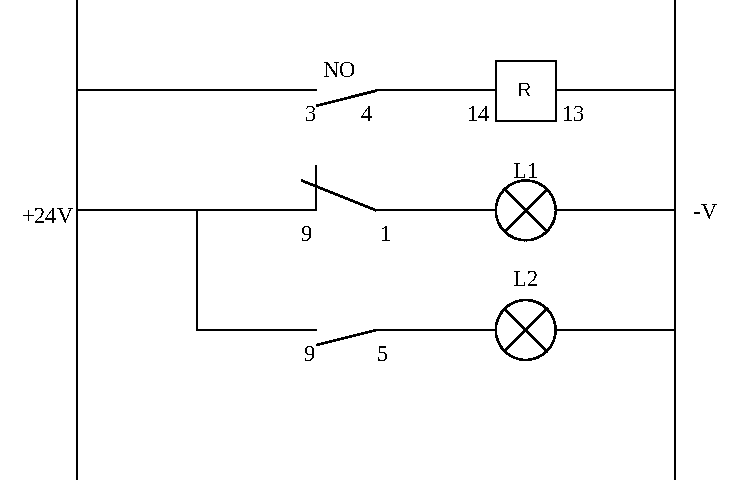
\includegraphics[scale=0.5]{sozai/1_compressed.pdf}
  \caption{リレー}
\end{figure}


\paragraph{課題1-1 自己保持回路}
a接点スイッチだけではスイッチを押したときに出力はOFFとなってしまう.
SW1をONするとランプが点灯し,SW2をONにすると消灯する回路(自己保持回路)を作成せよ.\\
ヒント: SW1はa接点,SW2はb接点である.リレーを用いる.

\subsubsection{実験1-2 タイマ回路}
図1.2に示す回路で,電源を入れてからランプが点灯するまでの時間を計測し,
タイマ(型番: H3YN)の動作確認を行いなさい.ただし,タイマはソケットに装着し,
タイマ側面のモードをオンディレイに設定し,TIME RANGEは10sとする.
ディップスイッチはマイナスドライバーで設定すること.また,TIME RANGEを10sと変更し動作確認を行いなさい.
なお,設定時間は任意,自己保持せずにスイッチは押し続けてよいものとする.

\begin{figure}[H]
  \centering
  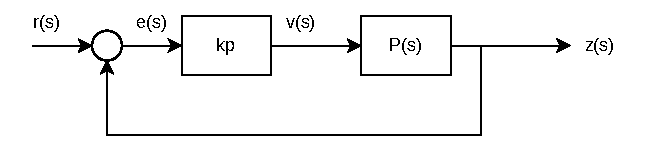
\includegraphics[scale=0.5]{sozai/2.pdf}
  \caption{タイマ回路}
\end{figure}

\subsubsection{実験1-3 タイマのモード}
タイマの各モードの動作を確認しなさい.
回路は実験1-3と同じでも構わない.

\paragraph{課題1-2 タイマ利用}
スイッチを一度押すことでランプを2つ自動で交互に点灯するような回路を作成せよ.
なお,自己保持回路を用いてタイマの起動を制御し,タイマのモードは適切に選択することで行うこと.\\

\paragraph{課題1-3 タイマ利用}
スイッチを一度押すとランプが点灯し,5秒後に自動消灯するような回路を作成せよ.
また自己保持回路を用いてタイマの起動を制御し,タイマのモードはオンディレイで行うこと.\\

\subsubsection{実験1-4 カウンタ回路}
図1.3に示す回路で,カウンタの動作確認を行いなさい.例えば,カウンタの設定値を5に設定後,
設定した値(5回)スイッチを押すたびにセンサが点灯するような回路を作成せよ.
また,リセットスイッチの効果を確認すること.\\
(注意)カウンタのピン番号の位置が実機とは異なる場合がある旨,表示に従って結線すること.

\begin{figure}[H]
  \centering
  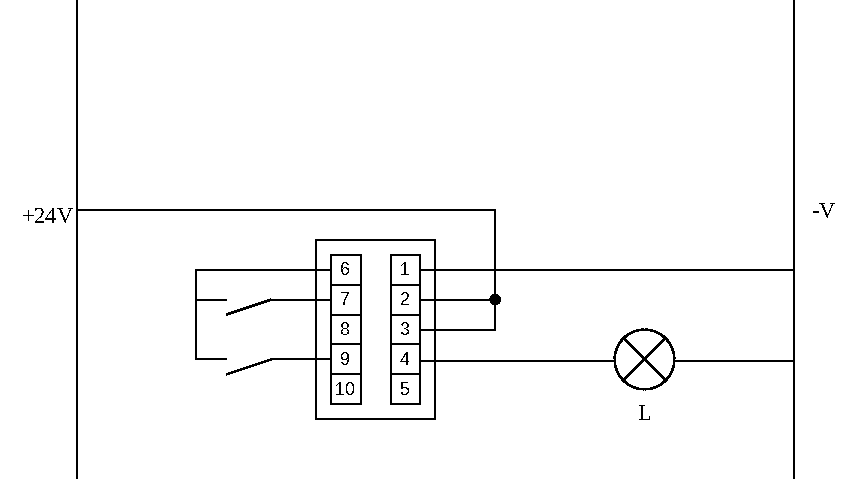
\includegraphics[scale=0.5]{sozai/3.pdf}
  \caption{カウンタ回路}
\end{figure}

\paragraph{課題1-4 カウンタとタイマ}
1秒につき1カウントする回路を作成せよ.ただし,起動には押しボタンスイッチを用いた自己保持回路を用いる.
また,カウンタのリセットについては考えなくてもよいものとする.
各機器のモードは適切なものを選択すること.\\
ヒント: タイマを用いる.

\subsubsection{実験1-5 センサを用いた回路}
図1.4に示す回路で,センサの動作確認を行いなさい.コンベアは「手動」に設定し,
角型9V乾電池とコンベアで運転しランプの点灯を確認する.センサは光電センサの中から好きなものを選んで,
コンベア周辺に取り付けること.

\begin{figure}[H]
  \centering
  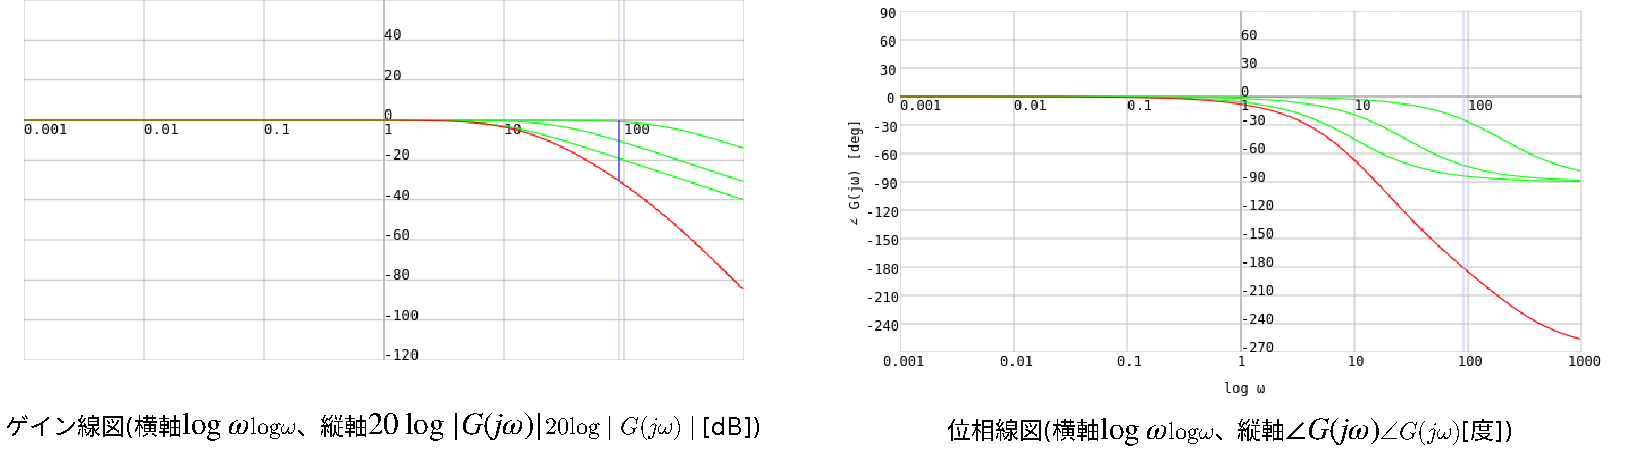
\includegraphics[scale=0.5]{sozai/4.pdf}
  \caption{センサを用いた回路}
\end{figure}

\paragraph{課題1-5 オートリセット回路}
設定数に達するとリセット入力を行うオートリセット回路を作成せよ.
カウンタの出力モードはNモードを用いること.また,カウンタは補助電極ON(自己保持回路は不要)とし,
カウントアップには押しボタンスイッチを用いること.

\paragraph{課題1-6 センサとカウンタ}
センサを用いたアップカウンタ回路を作成せよ.ただし,センサ,
カウンタ共に補助電極ON(自己保持回路は不要)とする.また,センサの選択は任意とする.
実験結果は実験1-8と同様に数値を記録するものとする.

\paragraph{課題1-7 複合回路}
センサ,リレー,タイマを用いて,コンベアでワークを運搬しセンサにかかるとコンベアを停止させ,
5秒後にコンベアを動き始める回路を作成せよ.


\section{PLCラダープログラムによる回路設計}

\subsection{実験目的}
第1節では,要求する動作に対してハードウェア(必要な部品とリード線)による物理的な結線で命令を実行してきた.
この方式はワイヤードロジックと呼ばれている.一方,要求する動作をプログラミングで実行する方式を
ソフトワイヤードロジックと呼び,この働きを持つ機器をPLC(Programmable Logic Controller)とする.
PLCを用いることで,回路の変更・更新が容易であり,
また回路を実際には作成しないため安価であるという利点がある.
第2節の本実験では,CX-Programmerというソフトウェアを用いてPLCのためのラダープログラムの設計について学ぶ.


\subsection{実験装置(プログラマブルロジックコントローラ)の説明}
PLCは入力部,演算制御部,出力部の3つに大別される.

PLCの主な機能は入出力機能である.例えば,入力部でセンサによる信号を受け,内部CPUで条件判断をし,
出力部のリレーを開閉することで接続されたモータをON/OFFするといった入出力機能を持つ.また,
CPU部でカウンタ,タイマ,内部補助リレー(仮想的なリレー)を有している点も特徴といえる.
表2.1にCPI1-Lの仕様を示す.入力リレーの個数は8点,出力リレーは6点,内部補助リレーは8192点
(正しくは他にもあるが省略する)となっている.これらのリレーにはアドレスと呼ばれる番号が付いている.

\begin{table}[h]
  \centering
  \caption{OMRON CP1L-Lの仕様}
  \begin{tabular}{|c|c|c|}
    \hline
    機能           & 点数    & アドレス       \\ \hline
    入力リレー     & 8点     & 0.00~0.07     \\ \hline
    出力リレー     & 6点     & 100.00~100.05 \\ \hline
    内部補助リレー & 8,192点 & W0.00~W511.15 \\ \hline
    タイマ         & 4,096点 & T0~T4095      \\ \hline
    カウンタ       & 4,096点 & C0~C4095      \\ \hline
  \end{tabular}
\end{table}

アドレスとは,そのリレーの場所を示す番号である.CP1L-Lは上段に入力端子,
下段に出力端子がある.本機では入力端子は0ch,出力端子は100chとあらかじめ決められている.
図2.3に入力端子とアドレスの関係を示す.入力端子は0chであると決まっているので,
アドレスは0.xxとなる.xxには接続する端子ごとに数字(ビット)が割り振ってある.
図2.3の例ではビット01および06なのでアドレスは0.01および0.06となる.

また,本実験ではそれほど多くの内部補助リレーを必要とはしないが,
1chごとのビット数は0~15までであることに注意する.つまり,16個の内部補助リレーW0.00~W0.15を使っていて,
もう1つ以上使いたい場合はW1.00以降となりW0.16は使えないことに注意する.

次に,入力部とCOMの関係について述べる.入力部とはスイッチやセンサなどの入力機器を接続し,
それらのON/OFF情報を取り込む部分である.COMに+24Vを接続し,
a接点をアドレス0.05に接続したとする.入力部の内部構造はフォトカプラとなっており,
入力部の端子とCOMとの電位差が生じることで入力がONと判断されることになる.
COM側が+24Vであってもフォトカプラは作動し,反対に端子側が+24Vであってもよい.ただし,
本実験で用いるセンサの検知信号は0V側と接続して用いる(第1節の1.4章を参考)ため
センサを用いるならばCOMを+24Vにする必要がある.また,センサの種類によって検知信号の電位は異なるという点に注意する.

次に,出力部とCOMの関係について述べる.出力部はランプやモーターなどの出力機器を接続し,
処理結果を外部出力するところである.PLCは内部リレー100.05をONとすることで
COMと端子05を導通させる機能を持つ.このためCOM端子に接続する電圧および方向は,
PLCに接続するモーターなどの出力機器に依存する.しかし,入力部のCOMは1つだけであったが,
出力部のCOMは出力端子ごとに個別となっている.これは出力機器がDC24V駆動であったり,
AC100V駆動であったりと様々であるため,それらに対応するためである.

\subsection{実験内容}

本実験では,「PLCラダープログラムによる回路設計」を行う.
以下に記載する実験2-1および課題2-1から2-8までを実施する.なお,
課題はラダープログラムを作成して動作確認を行うと共に,レポートにラダープログラム図を添付すること.

\subsubsection*{実験2-1 ラダープログラムの動作確認}
\begin{enumerate}
  \item ベーシックFAキットとPLCを配線する.\\
        PLCのIN端子00, 01, 02にNOスイッチ×3をそれぞれ接続する.\\
        そのNOスイッチを3-V, COMと+24V,およびPLCへの電源を接続する.
  \item 図2.9に示すようにプログラムをCX-Programmerで作成する.\\
        ソフトウェア上でNCの役割を行うことを確認する.
  \item 画面上で内部リレー(アドレスW1.00)が作動していることを確認する.
\end{enumerate}



\begin{figure}[H]
  \centering
  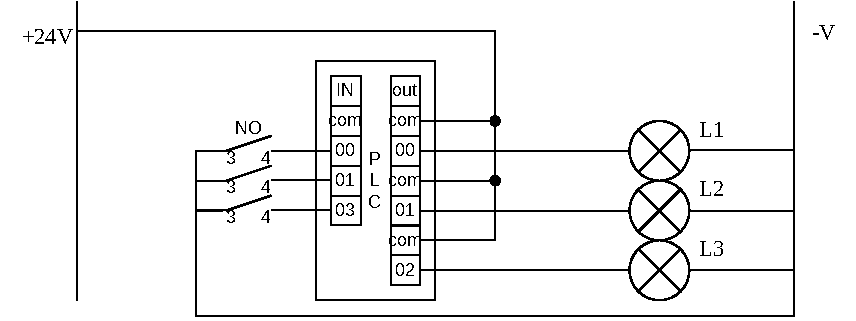
\includegraphics[scale=0.5]{sozai/5.pdf}
  \caption{ラダープログラムの動作確認のPLC}
\end{figure}

\subsubsection*{課題2-1 自己保持回路(課題1-1のラダープログラム)}
SW1をONするとランプが点灯し続け,SW2をONにすると消灯する回路(自己保持回路)を作成せよ.

\subsubsection*{課題2-2 タイマ利用(課題1-2のラダープログラム)}
スイッチを一度押すとランプが点灯し,5秒後に自動消灯するような回路を作成せよ.\\
ヒント:自己保持回路を用いてタイマの起動を制御.

\subsection*{課題2-3 タイマ利用(課題1-3のラダープログラム)}
スイッチを一度押すことでランプ2つを自動で交互に点灯させる回路を作成せよ.
ヒント:タイマを2つ使用するプログラムを以下に示す.これを改良して始動スイッチを設けること.

\subsubsection*{課題2-4 カウンタとタイマ(課題1-4のラダープログラム)}
1秒につき1カウントする回路を作成せよ.ただし,
起動には押しボタンスイッチを用いた自己保持回路を用いる.
また,通常のカウンタ(CNT)は減算であるため加減算カウンタ(CNTR)を用いること.
図2.11に示すようにCNTRには加算・減算・リセット信号の3つの信号を入力する必要がある.

\subsubsection*{課題2-5 オートリセット回路(課題1-5のラダープログラム)}
設定数に達するとリセット入力を行うオートリセット回路を作成せよ.ただし,
出力先が指定しないのでCX-Programmer上でカウンタがリセットされていることを確認すること.
条件:自己保持回路は不要とし,カウントアップには押しボタンスイッチを用いること.
カウンタはCNTを用いること.

\subsubsection*{課題2-6 センサとカウンタ(課題1-6のラダープログラム)}
センサを用いたアップカウンタ回路を作成せよ.カウンタには加減算カウンタCNTRを用いる.
また,実験体は実験1-8と同様に乾電池の通った数を数えるものとし,センサの種類は任意とする.
センサ等の起動に自己保持は用いなくてもよいものとする.

\subsubsection*{課題2-7 複合課題}
押しボタンスイッチ1つのみを用いて,一度押すとランプが点灯,
もう一度押すと消灯を繰り返すラダープログラムを作成せよ.
カウンタをCNTを用いた場合のラダーフローの流れを以下に示す.ただし,CNT,
CNTRどちらを用いてもよい.CNTRを使えば,タイマによりリセットの行程を省ける.

\subsubsection*{課題2-8 複合課題}
課題2-7を基に,押しボタンスイッチ1つでランプ2つを交互に点灯させる回路を作成せよ.ただし,
スイッチングする際(点灯する前)に1秒間のタイムラグを与えること.
つまり,
ランプ1点灯(X1秒)→ランプ1消灯→1秒経過→ランプ2点灯(X2秒)→ランプ2消灯→1秒経過→ランプ1点灯
の繰り返しとなる.
ここで,X秒のところは各自が押しボタンスイッチを押す間隔である.
また,スイッチを押すまではランプが点灯していないように工夫せよ.
